\documentclass[a4paper,12pt]{article}

\usepackage{geometry}
\geometry{top=15mm}
\geometry{bottom=30mm}
\geometry{left=10mm}
\geometry{right=20mm}
\linespread{1}
\setlength{\parindent}{12pt}
\setlength{\parskip}{8pt}

\usepackage{titleps}

\newpagestyle{main}
{
  \setheadrule{0.4pt}
  \sethead{}{}{}
  \setfootrule{0,4pt}
  \setfoot{}{\thepage}{}
}
\usepackage{color}
\usepackage[english,russian]{babel}
\usepackage[T2A]{fontenc}
\usepackage[utf8]{inputenc}
\usepackage{amsthm,amsmath,amsfonts,amssymb,mathtools}
\usepackage{indentfirst}
\usepackage{lipsum}
\usepackage{graphicx}
\usepackage{float}

\begin{document}
  
  \section*{Задача 1}

  Первая задача имеет три подпункта:
  \begin{itemize}
    \itemВычисление машинного $\epsilon$. \n В основе алгоритма лежит увеличение числа вдвое до тех пор, пока условие не станет истинным, а затем асимптотическое приближение к искому числу регулируемым шагом.\nВычисления показали, что $\epsilon = 5.960464e-008$, для переменной типа $float$, и $\epsilon=1.110223e-016$ для переменной типа $double$.
    \itemВычисление минимального числа A, такого что $A+1=A$.\n В основе лежит тот же подход, что и выше. Вычисления показывают, что $A=9.007199e+015$.
    \itemВычисление минимального числа А, такого что $A+10^{20}==A$.\n Применяем все тот же алгоритм. Вычисления показывают, что $A=1.329228e+036$.
  \end{itemize}
    \pagebreak[1]
  \section*{Задача 2}
  В этой задаче нам нужно было расчитать следующий интеграл:
  $$I_n = \int_{0}^{1} \frac{x^n}{x+6} dx$$
  Нам необходимо посчитать $I_{31}$. Это возможно сделать несколькими путями:
  \begin{itemize}
    \itemПосчитаем $I_0=ln(\frac{6}{7})$, и используя рекурентное соотношение $I_n=\frac{1}{n}-6*I_{n-1}$, посчитаем $I_{31}$. Получаем результат $I_{31}=-5.884485e+007$. Этот результат дает огромную погрешность по следующей причине. На самом деле компьютер не может реально хранить число $ln(\frac{6}{7})$, поэтому в памяти лежит лишь часть бесконечной непереодической десятичной записи этого числа. При каждой итерации вычисления рекурентного соотношения это ошибка множится на 6, таким образом эта погрешность увеличивается порядка $О(6^n)$.
    \itemИзвестно, что $I_{60}\simeq0$, поэтому учитывая точность записи числа, допустимо положить $I_{60}=0$. Затем повторно воспользоваться рекурентным соотношением. Этот способ дает результат $I_{31}=4.483776e-003$.
    \itemНаконец последний способ, это получить интеграл с помощью сумм Римана,то есть посчитать следующую сумму: $$\sum_{i=0}^{999} \frac{1}{1000}*f(i*\frac{1}{1000}+\frac{1}{1000}).$$ Получим $I_{31}=4.555572e-003$, при 1000 шагах. При 10000 шагах получаем $I_{31}=4.490923e-003$.
  \end{itemize}
\newpage
  \section*{Задача 3}
  В математике производная определяется следующим образом:$ f'(x)=\lim\limit_{h\rightarrow 0+} \frac{f(x+h)-f(x)}{h}$. Оказывается такое определение с вычислительной точки зрения некорректно.\n  Это связано с тем, что в оценке на точность появляется слогаемое $\frac{\epsilon}{h}$, которое стремится к бесконечности со стремлением h к 0. Проверяем это явным образом, а именно расcчитываем $R=f'(x)-\frac{f^*(x+h)-f^*(x)}{h}$  в зависимости от  $h$, где $f(x)=5 \sin(x)+x^2-e^x$. Получаем следующую таблицу:
  \begin{table}[h]
    \begin{center}
      \begin{tabular}{|c|c|c|c|c|c|c|}
      \hline
      &$h$&$R$&$h$&$R$&$h$&$R$ \\
      \hline
      1&9.090909e-015&4.725704e-001&3.376040e-015&9.588006e-001&1.253741e-015&6.165155e-001\\
      \hline
      2&8.576329e-015&3.944107e-001&3.184944e-015&7.248437e-002&1.182775e-015&4.886236e-001\\
      \hline
      3&8.090877e-015&3.736984e-001&3.004664e-015&1.065297e+000&1.115825e-015&1.660071e+000\\
      \hline
      4&7.632903e-015&1.848849e-001&2.834588e-015&1.488687e+000&1.052665e-015&3.848135e+000\\
      \hline
      5&7.200851e-015&2.872833e-001&2.674140e-015&4.358782e-001&9.930805e-016&2.936893e+000\\
      \hline
      6&6.793256e-015&4.698317e-001&2.522774e-015&6.800991e-001&9.368684e-016&1.970976e+000\\
      \hline
      7&6.408732e-015&7.417795e-001&2.379975e-015&1.122470e+000&8.838381e-016&9.471051e-001\\
      \hline
      8&6.045974e-015&3.558437e-001&2.245260e-015&4.768817e-002&8.338095e-016&1.381986e-001\\
      \hline
      9&5.703749e-015&2.735774e-001&2.118169e-015&1.091581e+000&7.866127e-016&1.288620e+000\\
      \hline
      10&5.380895e-015&2.184927e-001&1.998273e-015&2.145525e+000&7.420875e-016&2.508068e+000\\
      \hline
      11&5.076316e-015&4.891935e-001&1.885163e-015&1.132126e+000&7.000825e-016&3.800682e+000\\
      \hline
      12&4.788978e-015&6.235849e-001&1.778456e-015&5.792399e-002&6.604552e-016&1.096672e+001\\
      \hline
      13&4.517903e-015&5.559602e-001&1.677789e-015&1.080731e+000&6.230710e-016&1.048259e+001\\
      \hline
      14&4.262173e-015&5.528122e-001&1.582819e-015&2.287704e+000&5.878028e-016&9.969414e+000\\
      \hline
      15&4.020918e-015&3.900488e-002&1.493226e-015&3.570565e+000&5.545309e-016&9.425449e+000\\
      \hline
      16&3.793319e-015&1.100785e+000&1.408704e-015&2.642669e+000&5.231424e-016&8.848846e+000\\
      \hline
      17&3.578603e-015&1.729523e-001&1.328966e-015&1.659099e+000&4.935306e-016&8.237646e+000\\
      \hline
      \end{tabular}
    \end{center}
  \end{table}

Эти данные удобно указать в виде графика:
      \begin{figure}[H]
        \centering
          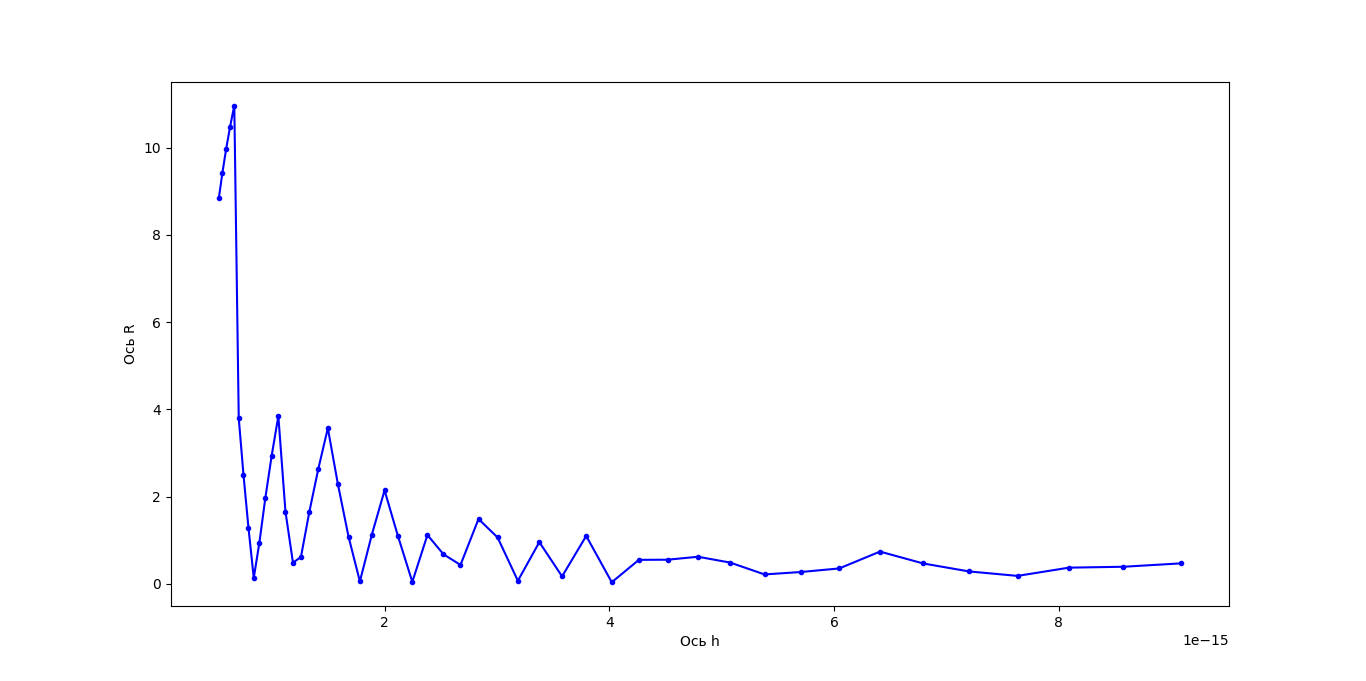
\includegraphics[width=0.8\textwidth, height=10cm]{DEF_3.png}
      \end{figure}
      
\newpage
  \section*{Задача 4}
  В этой задаче мы хотим реализовать метод Эйлера.
  Допустим у нас имеется уравнение вида $\dot y=f(t)$, а также начальное условие $y(0)=0$. А нам необходимо узнать $y(10)$.
  Предположим, что функция достаточно гладкая, тогда по формуле Ньютона-Лейбница имеем $\int_{0}^{10}f(t)dt=y(10)-y(0)$, то есть $y(10)=y(0)+\int_{0}^{10}f(t)dt$.
  Метод Эйлера заключается в первом приблежении такого вычисления, а имеено считая, что $\int_{x_0}^{x_0+h}f(t)dt\rightarrow f(x_0)\cdot h$,при $h\rightarrow0$, положим  $y(x_0+h)=y(x_0)+f(x_0)\cdot h$. После рекурентно посчитаем $y(10)$, считая шаг $h$ заданным. Метод тем точнее, чем меньше число $h$.
  Так, например, сделаны расчеты для двух функций: 
  \begin{align*}
    f_1(t)=\frac{e^t}{e^8}+cox(t)\cdot10+\frac{2t}{10}, \\
    F_1(t)=\frac{e^t-1}{e^8}+sin(t)\cdot10+\frac{t^2}{10}
  \end{align*}
  а также
  \begin{align*}
    f_2(t)=t, \\
    F_2(t)=\frac{t^2}{2}.
  \end{align*}
  \begin{figure}[H]
    \begin{flushleft}
      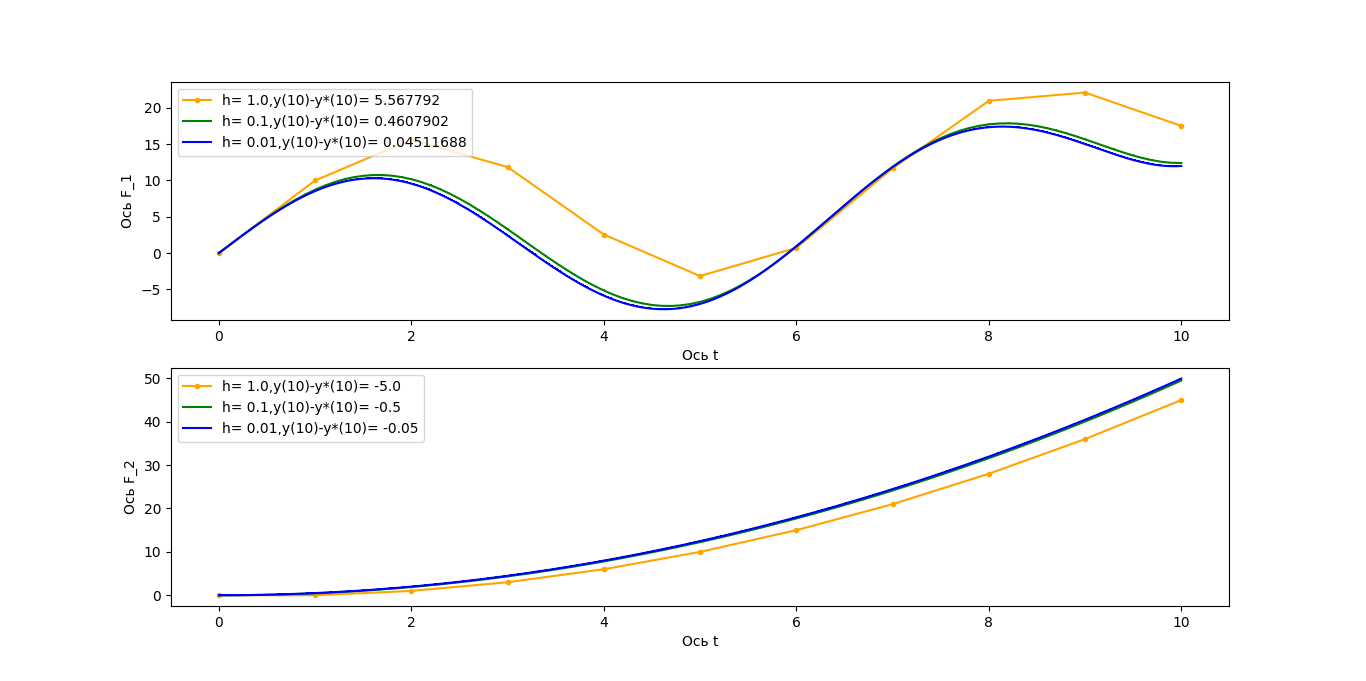
\includegraphics[width=1.0\textwidth, height=14cm]{DEF_4.png}
    \end{flushleft}
  \end{figure}
  
  
\newpage
  \section*{Задача 5}

  Теперь рассмотрим уравнение гармонического осциллятора:
  \begin{align*}
    \left\{
      \begin{array}{c}
        \dot x=y
        \\
        \dot y=-x
      \end{array}
    \right.
  \end{align*}
  
  Попытаемся решить это уравнение с помощью метода Эйлера. То есть используя следующее рекурентное соотношение:

  \begin{align*}
    \left\{
      \begin{array}{c}
        x(x_0+h)=x_0+y_0 \cdot h
        \\
        y(x_0+h)=y_0-x_0 \cdot h
      \end{array}
    \right.
  \end{align*}
  
  \begin{table}[htb]
    \begin{center}
      \begin{tabular}{|c|c|c|c|c|c|c|}
      \hline
      &$h=0.1$&&$h=0.01$&&$h=0.001$&\\
      \hline
      $T$&$x(T)-sin(T)$&$y(T)-cos(T)$&$x(T)-sin(T)$&$y(T)-cos(T)$&$x(T)-sin(T)$&$y(T)-cos(T)$\\
      \hline
      $\pi$&1.202282e-02&-1.677062e-01&1.063179e-04 &-1.582438e-02&1.048714e-06 &-1.571909e-03\\
      \hline
      $10\pi$&-4.938385e-01&3.737179e+00&-1.225010e-03 &1.700568e-01&-1.063754e-05 &1.583174e-02\\
      \hline
      $10^2\pi$&-5.277214e+06&3.093268e+06&-5.036450e-02&3.809691e+00&-1.225303e-04&1.700883e-01\\
      \hline
      $10^3\pi$&6.289921e+67&-4.178951e+67&-6.929947e+05&6.593824e+06&-5.038380e-03&3.810469e+00\\
      \hline
      $10^4\pi$&nan&nan&-1.421995e+68&8.211133e+67&-6.952562e+04&6.635203e+06\\
      \hline
      $10^5\pi$&nan&nan&nan&nan&-1.700005e+67&1.646191e+68\\
      \hline
      $10^6\pi$&nan&nan&nan&nan&nan&nan
      \\
      \hline
      \end{tabular}
    \end{center}
  \end{table}
  
  \FloatBarrier
  Как видим, с уменьшением шага растет точность результатов. Так, например, некоторое представление дают следующие графики:

\begin{figure}[H]
      \centering
      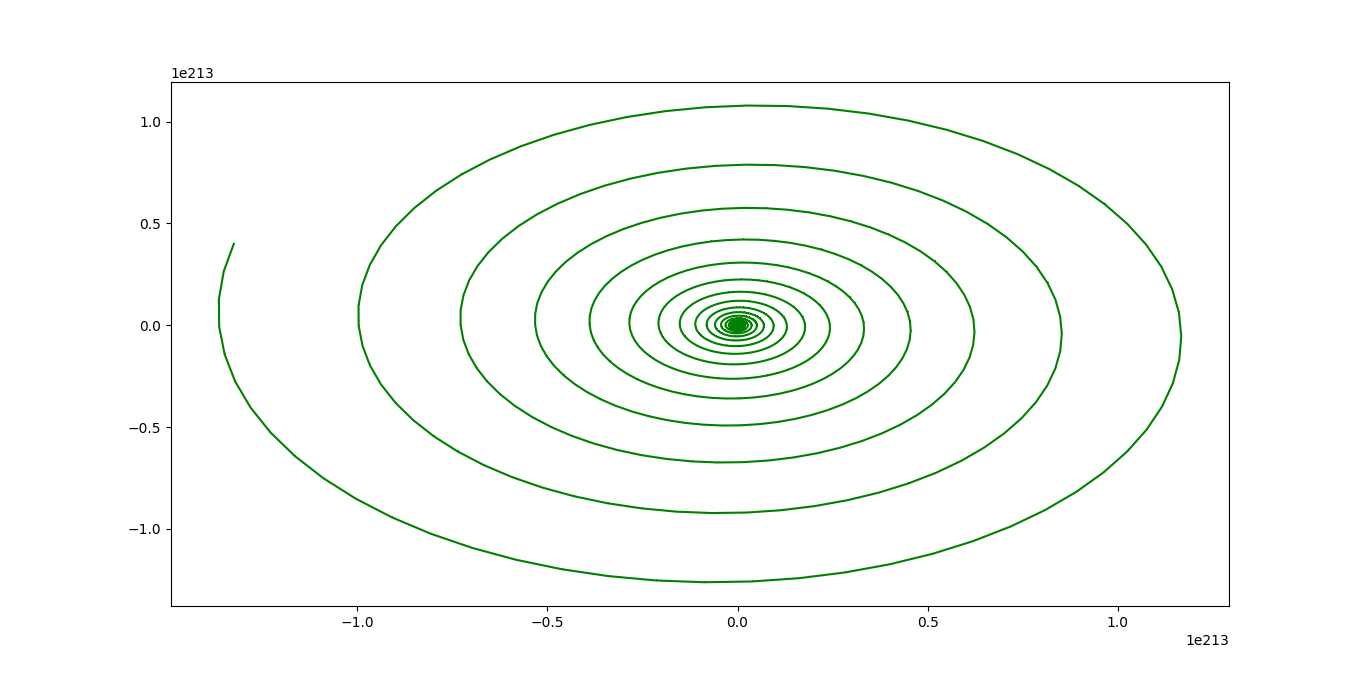
\includegraphics[width=0.7\textwidth]{DEF_5_1.png}
      \caption{Изображение с оборотами около 980 $\pi$.}
      
\end{figure}
\begin{figure}
\centering
      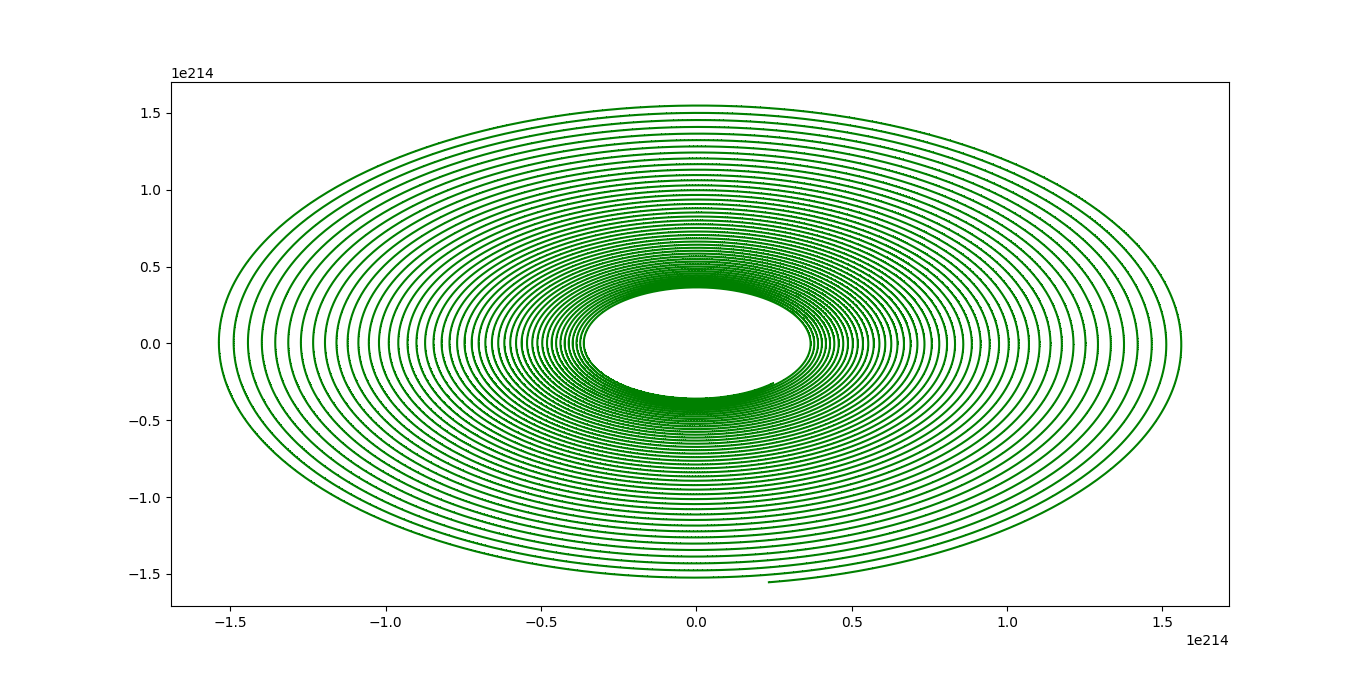
\includegraphics[width=0.7\textwidth]{DEF_5_2.png}
      \caption{Изображение с оборотами около 9980 $\pi$.}
\end{figure}
\begin{figure}
\centering
      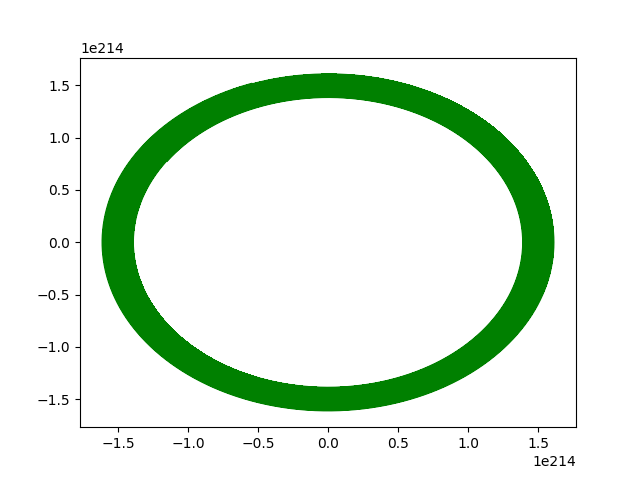
\includegraphics[width=0.7\textwidth]{DEF_5_3.png}
      \caption{Изображение с оборотами около 99980 $\pi$.}
  \end{figure}
  \FloatBarrier

  \newpage

  \section*{Задача 6}
  Теперь применим более тонкий алгоритм в задаче гармонического осциллятора.
  Применяя алгоритм Рунге-Кутта мы сильно выиграем в точности. Используя коэффициенты из таблицы Дорман-Принс 5(4), получим следующую таблицу результатов, из которой видно колоссальный разрыв в точности:
    \begin{table}[htb]
      \begin{center}
        \begin{tabular}{|c|c|c|c|c|c|c|}
			\hline
			&$h=0.1$&&&$h=0.01$&&\\
			\hline
			$T$&$x(T)-sin(T)$&$y(T)-cos(T)$&$err_{global}$&$x(T)-sin(T)$&$y(T)-cos(T)$&$err_{global}$\\
			\hline
			$\pi$&-1.472467e-09&8.515779e-09&2.253933e-07&-2.472301e-14&8681944e-14&2.285026e-11\\
			\hline
			$10\pi$&1.487203e-08&-8.601541e-08&2.279565e-06&-2.099069e-12&-8.743006e-13&2.285874e-10\\
			\hline
			$10^2\pi$&1.491395e-07&-8.624701e-07&2.285896e-05&1.408575e-10&-8.731016e-12&2.286244e-09\\
			\hline
			$10^3\pi$&1.493784e-06&-8.628065e-06&2.286836e-04&-2.215149e-08&-8.724321e-11&2.286302e-08\\
			\hline
			$10^4\pi$&1.509647e-05&-8.628162e-05&2.286867e-03&2.094986e-06&-8.746502e-10&2.286312e-07\\
			\hline
			$10^5\pi$&1.504219e-04&-8.624965e-04&2.285993e-02&-1.405452e-04&-1.860093e-08&2.286313e-06\\
			\hline
			$10^6\pi$&-2.823716e-04&-8.591500e-03&2.277143e-01&2.154231e-02&-2.321498e-04&2.286313e-05\\
			\hline
        \end{tabular}
      \end{center}
    \end{table}
    \FloatBarrier

    \begin{table}[htb]
      \begin{center}
        \begin{tabular}{|c|c|c|c|}
			\hline
			&$h=0.001$&&\\
			\hline
			$T$&$x(T)-sin(T)$&$y(T)-cos(T)$&$err_{global}$\\
			\hline
			$\pi$&-1.472467e-09&8.515779e-09&3.616248e-15\\
			\hline
			$10\pi$&1.487203e-08&-8.601541e-08&3.355828e-14\\
			\hline
			$10^2\pi$&1.491395e-07&-8.624701e-07&3.112587e-13\\
			\hline
			$10^3\pi$&1.493784e-06&-8.628065e-06&3.122459e-12\\
			\hline
			$10^4\pi$&1.509647e-05&-8.628162e-05&3.142585e-11\\
			\hline
			$10^5\pi$&1.504219e-04&-8.624965e-04&3.140465e-10\\
			\hline
			$10^6\pi$&-2.823716e-04&-8.591500e-03&3.139796e-09\\
			\hline
        \end{tabular}
      \end{center}
    \end{table}
    \FloatBarrier

	\section*{Задача 7}
	В этой задаче мы реализуем алгоритм Рунге-Кутта с коэффициентами из таблицы  Дорман-Принс 5(4) с автоматическим выбором шага.
	Суть его в следующем, согласно алгоритму высчитывается пара значений, по которым получается глобальная погрешность $err.$. Эта погрешность сравнивается с допустимой глобальной погрешностью для шага $tol.$  Если $err<tol$, то шаг засчитывается, после чего происходит пересчет длины шага $h$. Если же погрешность больше $tol$, то шаг игнорируется, после чего происходит изменение его длины.
	\[h_{new}=h*min(facmax,max(facmin,fac*( \frac{tol}{err})^{\frac{1}{p+1}} ))\]

	Например, применяя этот алгоритм для задачи о гармоническом осцилляторе, получается таблица данных:

	\begin{table}[H]
		\begin{center}
		  \begin{tabular}{|c|c|c|c|c|c|c|}
			  \hline
			  &$tol=10^{-9}$&&$tol=10^{-11}$&&$tol=10^{-13}$&\\
			  \hline
			  $T$&$x(T)-sin(T)$&$y(T)-cos(T)$&$x(T)-sin(T)$&$y(T)-cos(T)$&$x(T)-sin(T)$&$y(T)-cos(T)$\\
			  \hline
			  $\pi$&-6.566687e-11&6.419453e-10&-2.595161e-13&6.442846e-12&-1.202547e-15&6.439294e-14\\
			  \hline
			  $10\pi$&6.549747e-10&-6.407378e-09&2.528302e-12&-6.421508e-11&4.492970e-14&-6.428191e-13\\
			  \hline
			  $10^2\pi$&6.556711e-09&-6.412660e-08&2.633449e-11&-6.431748e-10&-1.883722e-15&-6.429857e-12\\
			  \hline
			  $10^3\pi$&6.558337e-08&-6.413007e-07&2.505577e-10&-6.434210e-09&1.552589e-10&-6.436629e-11\\
			  \hline
			  $10^4\pi$&6.553341e-07&-6.413426e-06&2.529095e-09&-6.434469e-08&1.254655e-09&-6.437467e-10\\
			  \hline
			  $10^5\pi$&6.573922e-06&-6.413481e-05&5.032478e-08&-6.434508e-07&-3.204558e-08&-6.436897e-09\\
			  \hline
			  $10^6\pi$&6.600483e-05&-6.413505e-04&1.281037e-06&-6.434511e-06&2.470806e-06&-6.437168e-08\\
			  \hline
		  \end{tabular}
		\end{center}
		\caption{Использовались параметры $p=5 ,fac=0.9 ,facmax=1.3 ,facmin=0.7$.}
	  \end{table}
	  \FloatBarrier

	  Заметим лишь, что для точностей $tol=10^{-9}$ и $tol=10^{-11}$ получим $h=O(10^{-2})$, а для точности $tol=10^{-13}$ получим $h=O(10^{-3}).$

	Этот же алгоритм можно применить, например, к следующей системе:
	\begin{align*}
	\left\{
		\begin{array}{c}
		\dot x=-20( sin(50\cdot t)\cdot50\cdot e^{-4t} + 4\cdot e^{-4t}cos(50\cdot t))
		\\
		x(0)=0.
		\end{array}
	\right.
	\end{align*}
	Здесь мы для яркости представления регулировки длины шага используем следующие параметры $p=5, fac=0.9, facmax=10, facmin=0.7.$
	
	\begin{figure}[H]
	\centering
			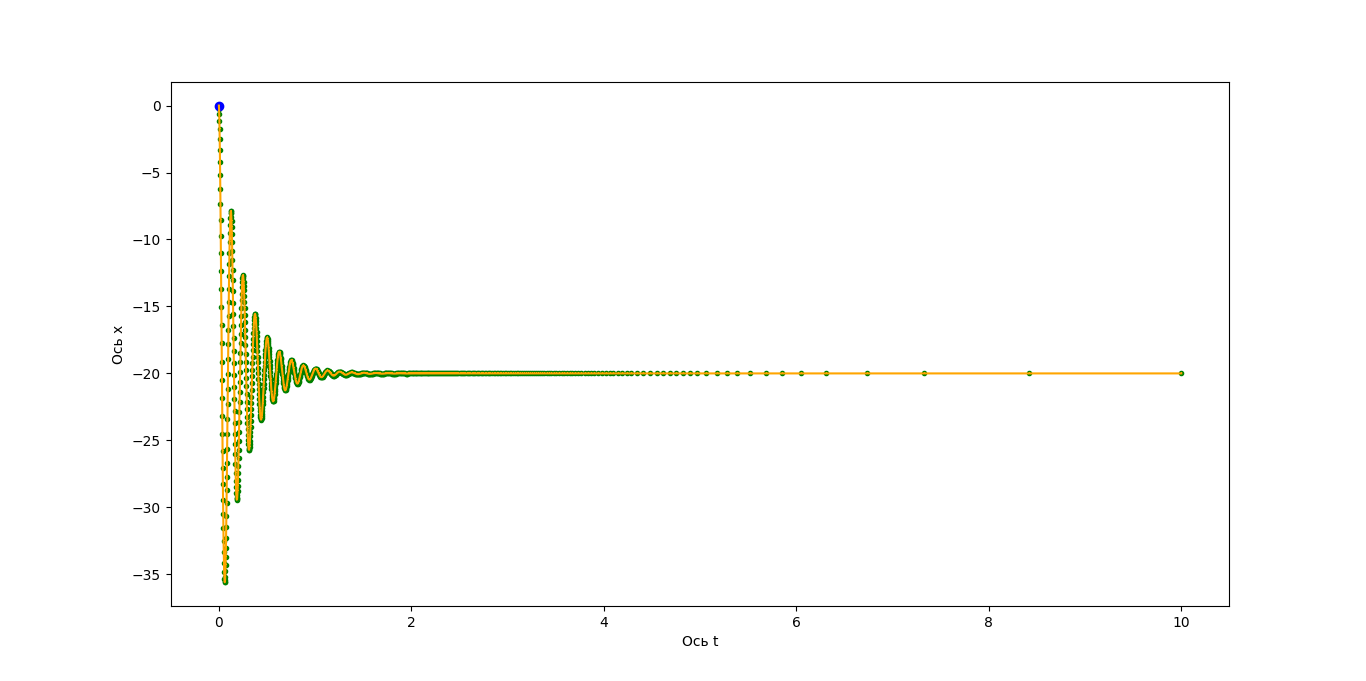
\includegraphics[width=1\textwidth]{DEF_7_1.png}
	\end{figure}
	
	
	\section*{Задача 8}
	Теперь решаем задачу о поиске переодических уравнений системы. Задача имеет вид:
	\begin{align*}
	\left\{
		\begin{array}{c}
		\frac{dx}{dt}=y
		\\
		\frac{dy}{dt}=\alpha \cdot (1-x^2) \cdot y - x
		\end{array}
	\right
  \\
  \alpha \in {0.1 , 10.0}
	\end{align*}

	Для начала попытаемся приблизительно узнать, как выглядит цикл, то есть переодическое решение. Для этого зададим начальные условия так, чтобы они не совпали с особыми точками $(y=0,x=0)$, и пустим из них нашу кривую, построенную по методу Рунге-Кутта с автоматическим выбором шага.

	Так при $\alpha = 0.1$ получим следующее изображение:
	\begin{figure}[H]
		\centering
				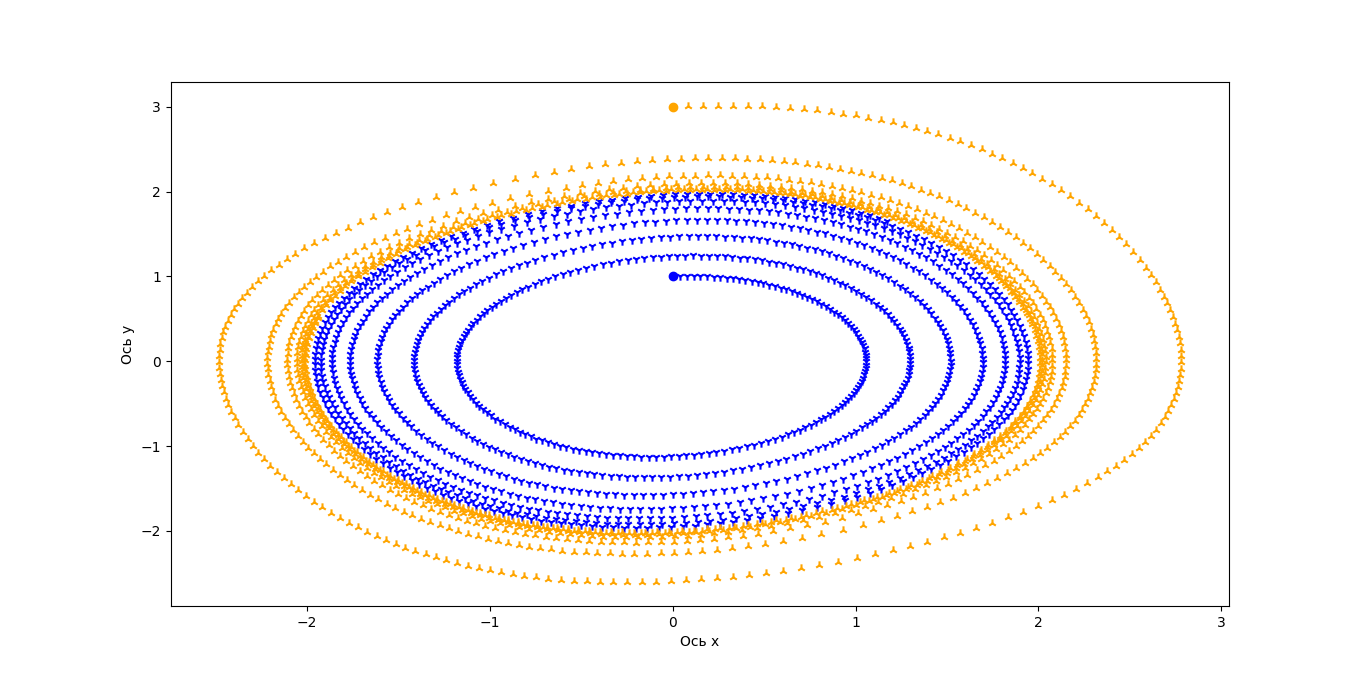
\includegraphics[width=1\textwidth]{DEF_8.png}
				\caption{Начальные условия: синий - $y=1, x=0$, оранжевый - $y=3, x=0.$}
	\end{figure}

	Так при $\alpha = 10.0$ получим следующее изображение:
	\begin{figure}[H]
		\centering
				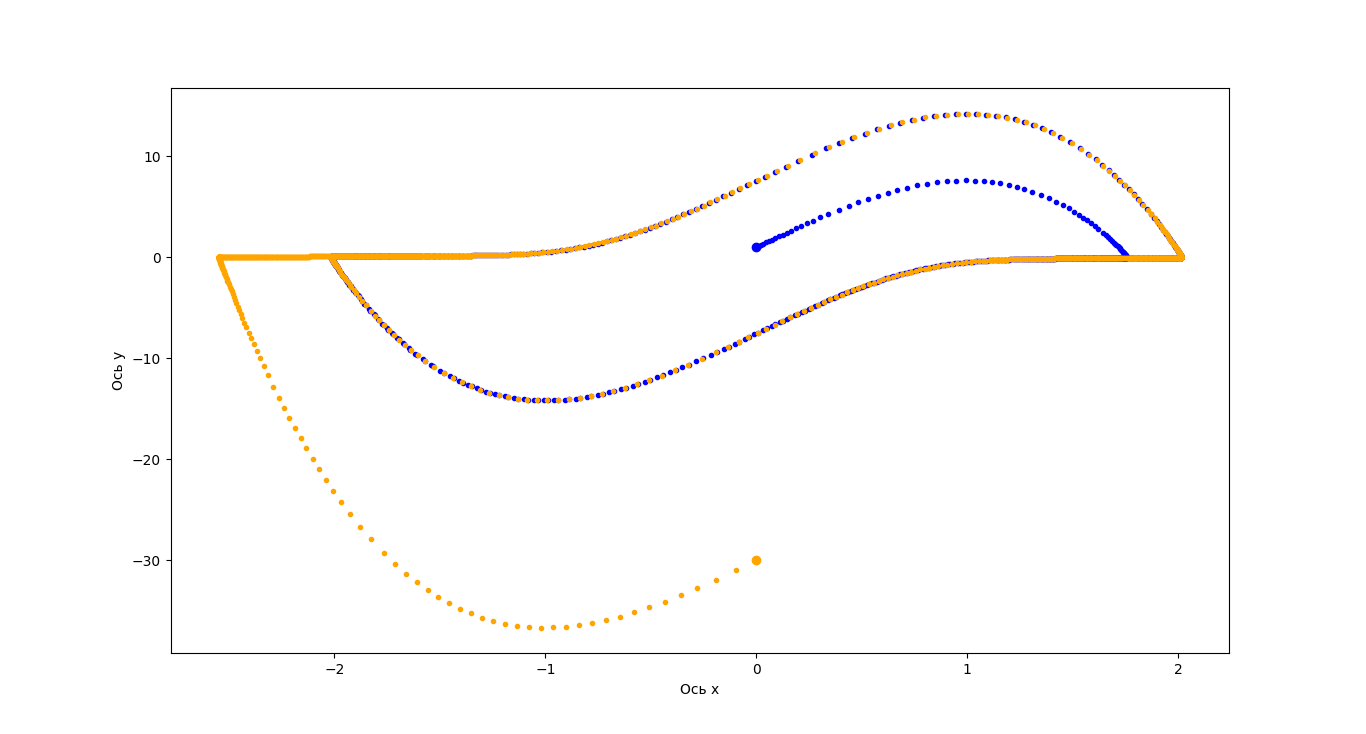
\includegraphics[width=1\textwidth]{DEF_8_1.png}
				\caption{Начальные условия: синий - $y=1, x=0$, оранжевый - $y=-30, x=0.$}
	\end{figure}

	Теперь, когда мы приблизительно знаем, как выглядят циклы, можно приступить к их поиску. Идея очень проста, берем неособенную точку и испускаем из нее вертикальный лучь. На этом луче выбираем точку и принимаем ее за начальные условия. После испускаем из этой точки решение, которое в итоге, совершив оборот, пересечет наш лучь.
	Конечно явного пересечения не будет, так как мы имеем лишь набор точек, поэтому будем искать точку пересечения методом хорд. Итак, найдя эту точку, мы можем оценить расстояние до точки на этом луче, с которой мы стартовали, если таковое расстояние будет меньше параметра $TOL$, считаем, мы нашли замкнутый цикл. Если это не так, то продолжаем иди по решению до следующего пересечения, и так далее...
	Конечно, пользуемся тем, что уже знаем, как приблизительно устроены решения. 

  Используем следующие параметры:\newline
  $tol=10^{-11}$ - максимальная погрешность при оценки допустимости следующего шага.\newline
  $Tol=10^{-11}$ - максимальная погрешность при оценки допустимости  выбора точки пересечения.\newline
  $TOL=10^{-9}$ - максимальная погрешность при оценки допустимости нахождения цикла.\newline

	\begin{figure}[H]
		\centering
				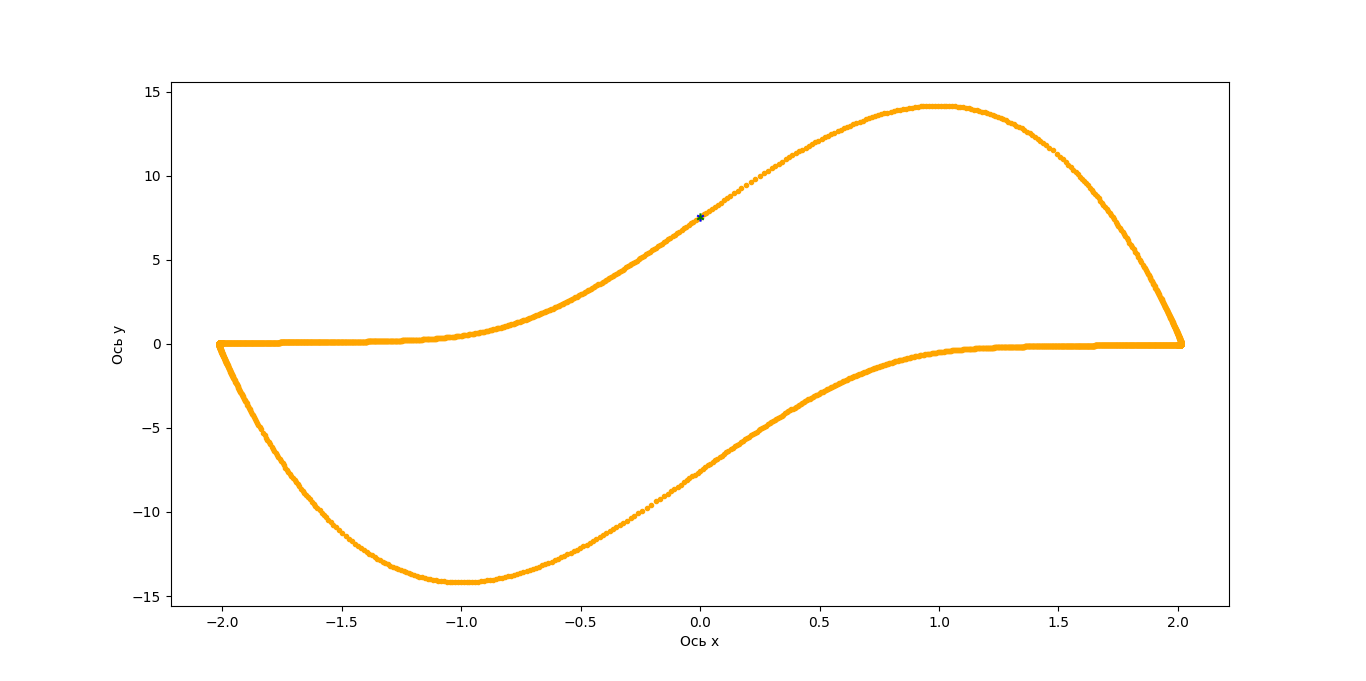
\includegraphics[width=0.8\textwidth]{DEF_8_3.png}
        \caption{$\alpha = 0.1$}
  \end{figure}

	\begin{figure}[H]
		\centering
				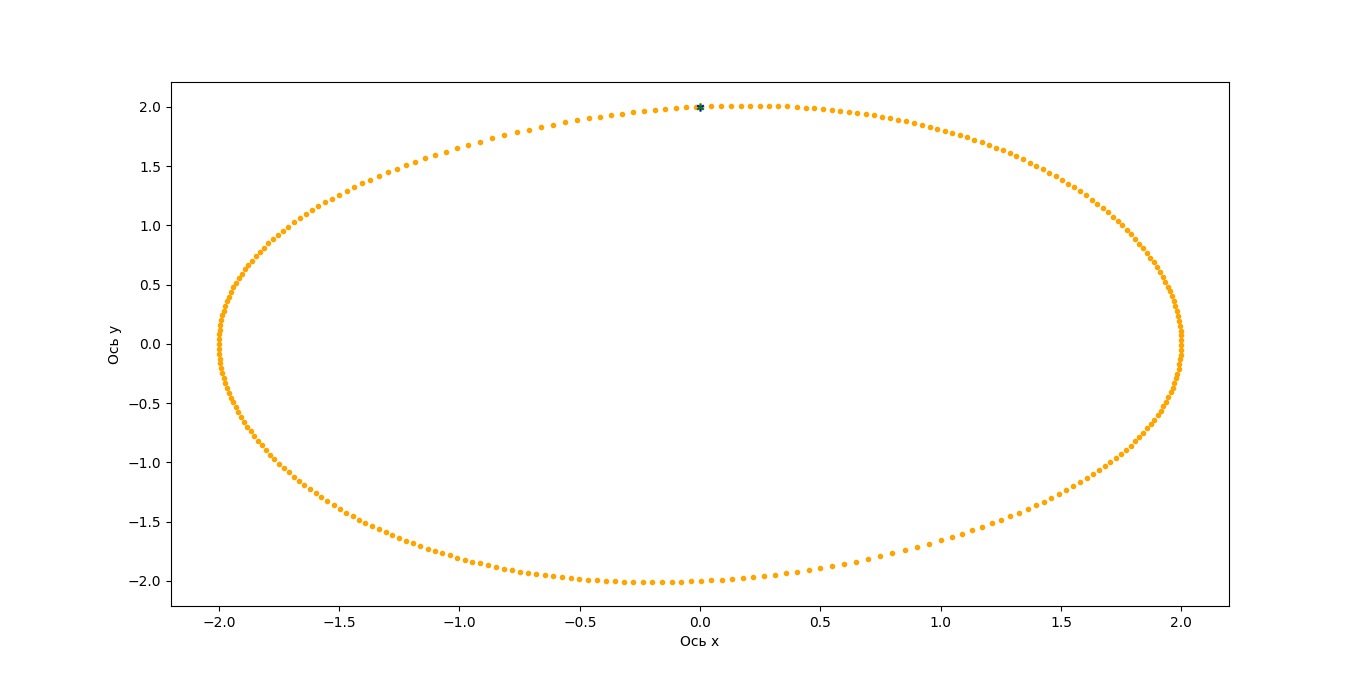
\includegraphics[width=0.8\textwidth]{DEF_8_4.png}
        \caption{$\alpha = 10.0$}
  \end{figure}

	\end{document}